% Native editable composition from verified, unchanged IDE images.
\par
\begin{figure}[htbp]
\centering
\sbox0{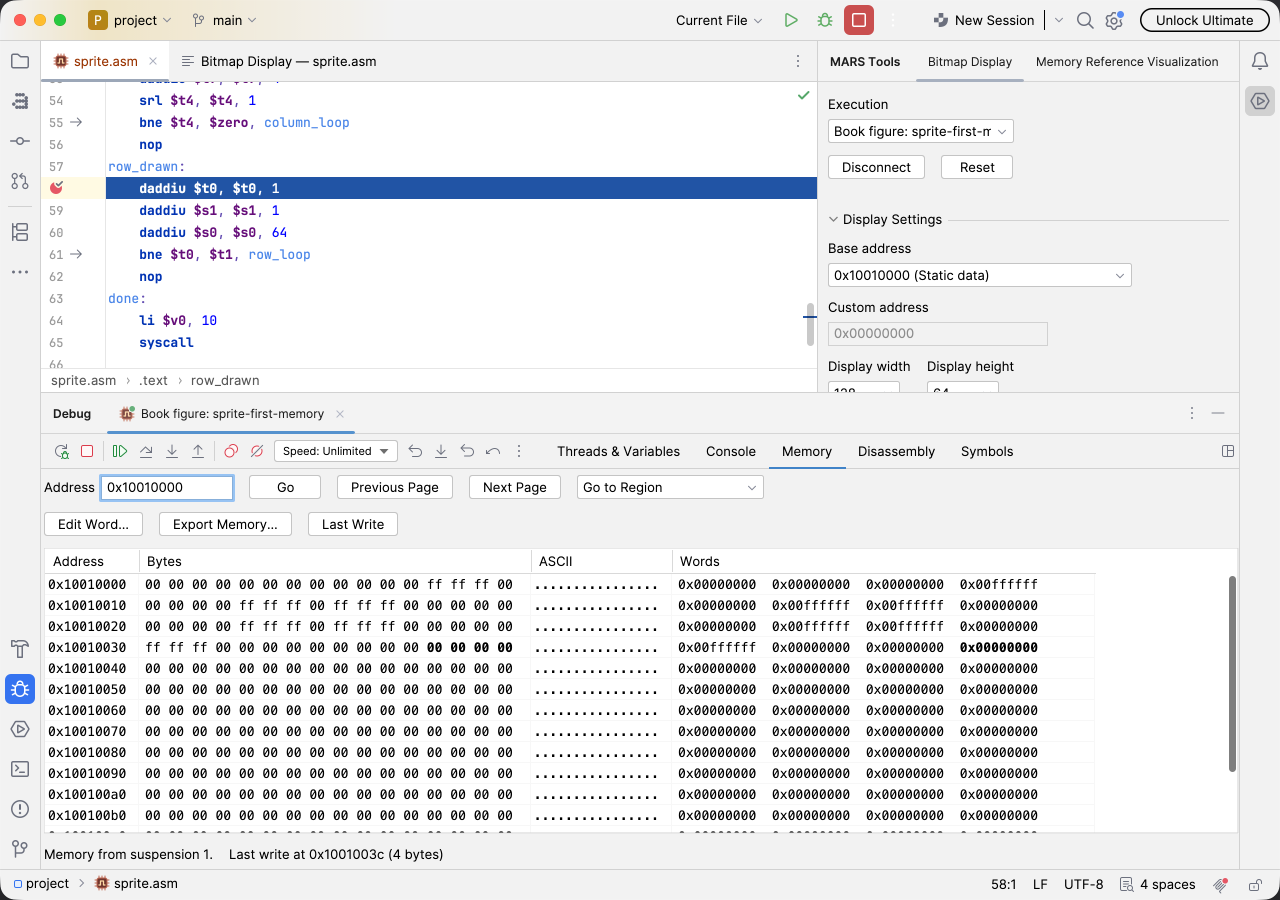
\includegraphics[artifact]{packages/003-eight-byte-sprite/captures/f03-first-row/memory.png}}
\sbox2{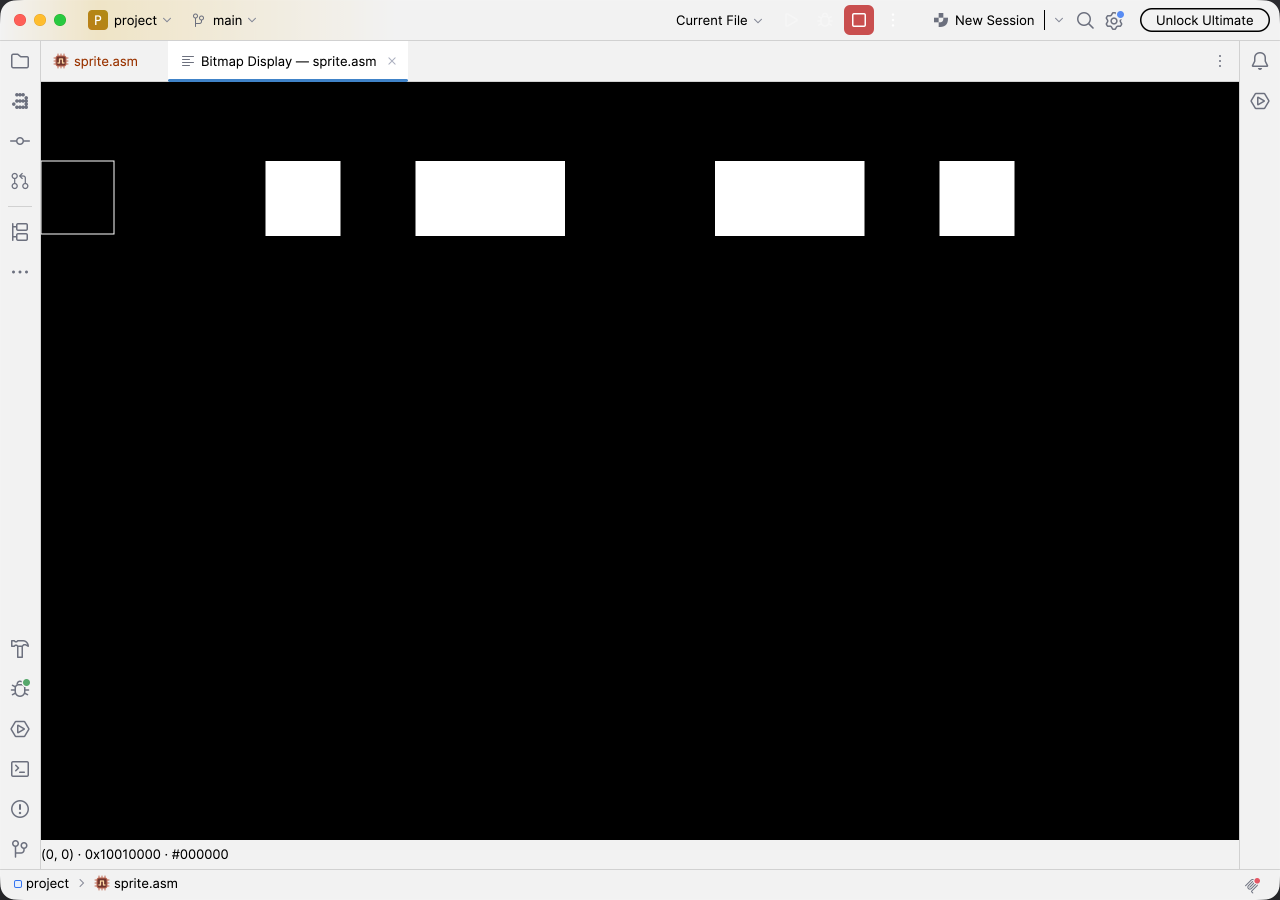
\includegraphics[artifact]{packages/003-eight-byte-sprite/captures/f03-first-row/bitmap.png}}
\edef\MARSfirstsourceLeft{\the\dimexpr0.036718750\wd0\relax}
\edef\MARSfirstsourceBottom{\the\dimexpr0.774444444\ht0\relax}
\edef\MARSfirstsourceRight{\the\dimexpr0.611718750\wd0\relax}
\edef\MARSfirstsourceTop{\the\dimexpr0.172222222\ht0\relax}
\edef\MARSfirstmemoryLeft{\the\dimexpr0.034375000\wd0\relax}
\edef\MARSfirstmemoryBottom{\the\dimexpr0.264444444\ht0\relax}
\edef\MARSfirstmemoryRight{\the\dimexpr0.578906250\wd0\relax}
\edef\MARSfirstmemoryTop{\the\dimexpr0.608888889\ht0\relax}
\edef\MARSfirstbitmapLeft{\the\dimexpr0.032031250\wd2\relax}
\edef\MARSfirstbitmapBottom{\the\dimexpr0.155555556\ht2\relax}
\edef\MARSfirstbitmapRight{\the\dimexpr0.032031250\wd2\relax}
\edef\MARSfirstbitmapTop{\the\dimexpr0.178888889\ht2\relax}
\begin{tikzpicture}[alt={Three annotated IDE details at the first row_drawn stop. The next instruction increments t0. The first 64 frame bytes contain sixteen little-endian black or white words. Across the first display row, the left eight cells are 00010110 and the right eight are 01101000, where one means white. The remaining seven display rows are black.}]
\node[anchor=north west,inner sep=0,font=\small\bfseries] (source-title) at (6mm,0) {The first row is complete};
\node[anchor=north west,inner sep=0] (source) at ([yshift=-1mm]source-title.south west) {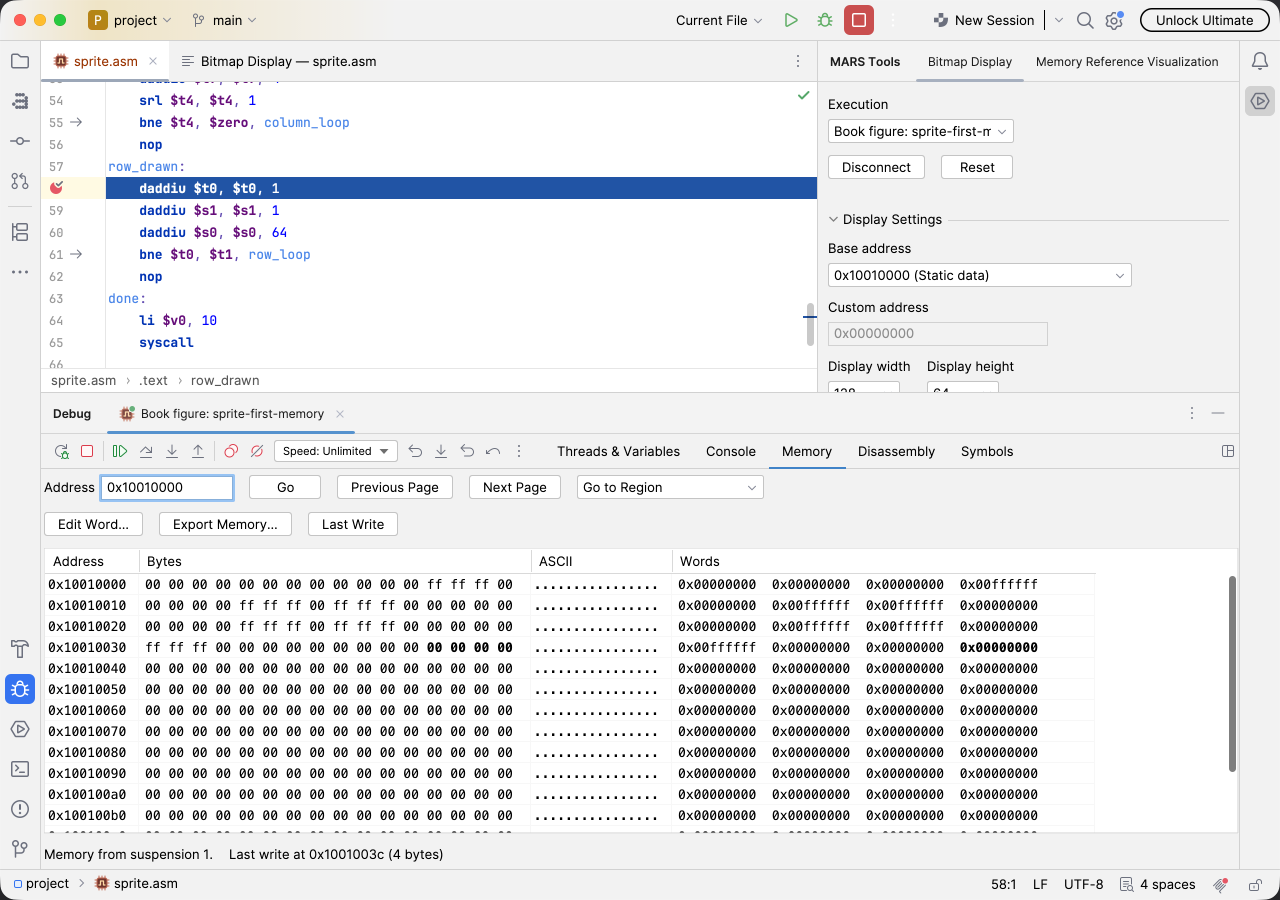
\includegraphics[width=0.7\linewidth,artifact,trim={\MARSfirstsourceLeft{} \MARSfirstsourceBottom{} \MARSfirstsourceRight{} \MARSfirstsourceTop{}},clip]{packages/003-eight-byte-sprite/captures/f03-first-row/memory.png}};
\begin{scope}[shift={(source.south west)},x={($(source.south east)-(source.south west)$)},y={($(source.north west)-(source.south west)$)}]
\draw[black,line width=0.7pt] (0.135555556,0.083333333) rectangle (0.515555556,0.541666667);
\node[draw=black,fill=white,circle,inner sep=1.5pt,font=\footnotesize] at ($(0.135555556,0.541666667)+(-3mm,0)$) {1};
\end{scope}
\node[anchor=north west,inner sep=0,font=\small\bfseries] (memory-title) at ([yshift=-2mm]source.south west) {Four memory rows hold sixteen pixel words};
\node[anchor=north west,inner sep=0] (memory) at ([yshift=-1mm]memory-title.south west) {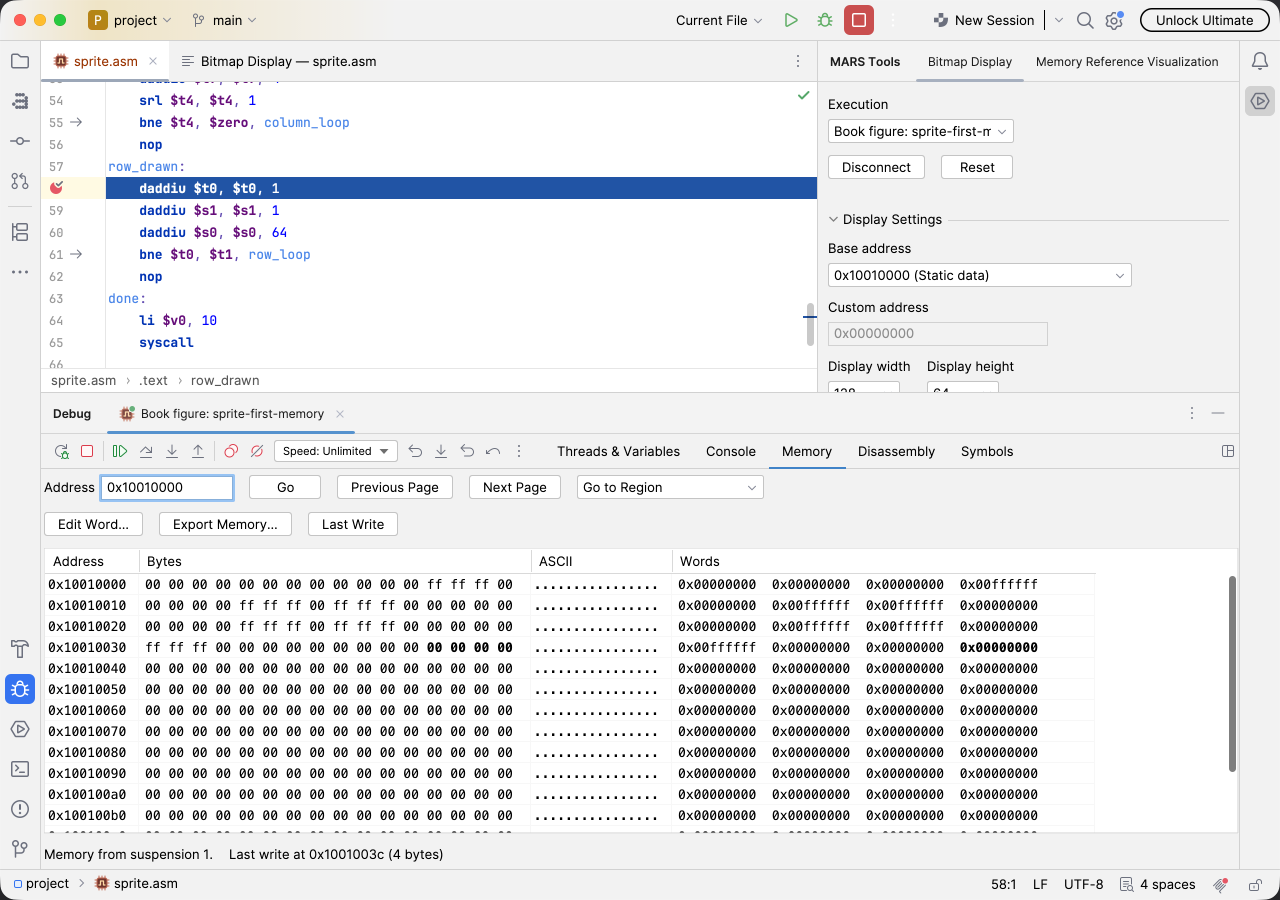
\includegraphics[width=0.84\linewidth,artifact,trim={\MARSfirstmemoryLeft{} \MARSfirstmemoryBottom{} \MARSfirstmemoryRight{} \MARSfirstmemoryTop{}},clip]{packages/003-eight-byte-sprite/captures/f03-first-row/memory.png}};
\begin{scope}[shift={(memory.south west)},x={($(memory.south east)-(memory.south west)$)},y={($(memory.north west)-(memory.south west)$)}]
\draw[black,line width=0.7pt] (0.191919192,0.035087719) rectangle (0.983838384,0.771929825);
\node[draw=black,fill=white,circle,inner sep=1.5pt,font=\footnotesize] at ($(0.191919192,0.771929825)+(-3mm,0)$) {2};
\end{scope}
\node[anchor=north west,inner sep=0,font=\small\bfseries] (bitmap-title) at ([yshift=-2mm]memory.south west) {Original and mirrored masks in the first display row};
\node[anchor=north west,inner sep=0] (bitmap) at ([yshift=-1mm]bitmap-title.south west) {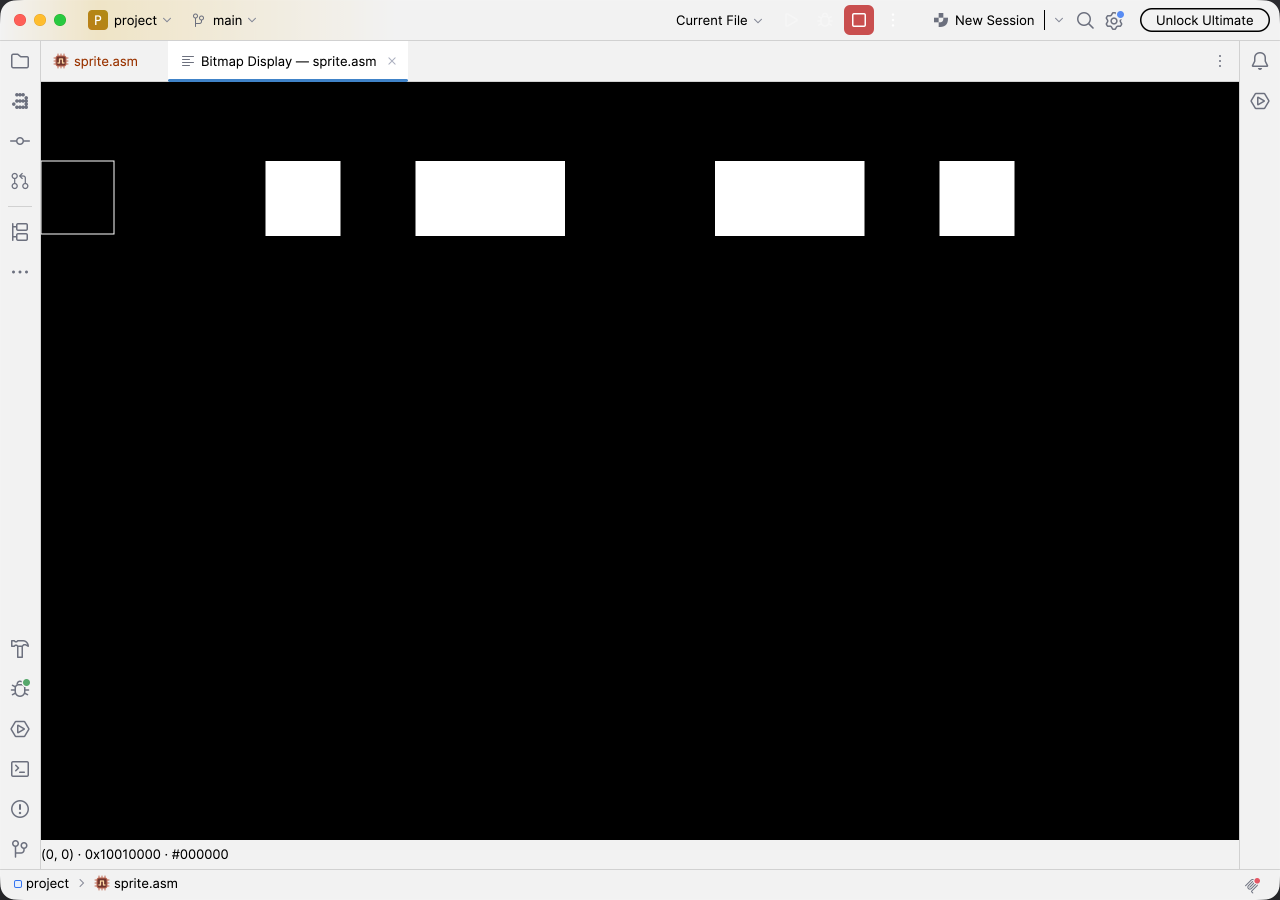
\includegraphics[width=0.84\linewidth,artifact,trim={\MARSfirstbitmapLeft{} \MARSfirstbitmapBottom{} \MARSfirstbitmapRight{} \MARSfirstbitmapTop{}},clip]{packages/003-eight-byte-sprite/captures/f03-first-row/bitmap.png}};
\begin{scope}[shift={(bitmap.south west)},x={($(bitmap.south east)-(bitmap.south west)$)},y={($(bitmap.north west)-(bitmap.south west)$)}]
\draw[black,line width=0.7pt] (0.000000000,0.000000000) rectangle (1.000000000,1.000000000);
\node[draw=black,fill=white,circle,inner sep=1.5pt,font=\footnotesize] at ($(0.000000000,1.000000000)+(-3mm,0)$) {3};
\end{scope}
\end{tikzpicture}
\par\smallskip
\begin{minipage}{\linewidth}
\small
\begin{enumerate}
\item Execution is paused before \texttt{daddiu \$t0, \$t0, 1}. The column loop has completed eight pairs of stores. The source pointer and frame-row pointer still identify the first row; the following instructions advance them.
\item Each displayed memory row contains four 32-bit pixels, so four memory rows hold one 16-cell display row. In this little-endian session, \texttt{ff ff ff 00} represents white \texttt{0x00ffffff}; \texttt{00 00 00 00} represents black. A memory-table row is not a display row.
\item The left eight cells read \texttt{00010110}; the right eight read \texttt{01101000}, with one meaning white. Only the top display row has been written. The seven black rows below it are still unprocessed at this stop. The thin outline on the upper-left cell is the display's hover marker, not a white pixel.
\end{enumerate}
\end{minipage}
\caption{After drawing one original row and its mirror. Two native Debug views share the stop before advancing the row pointers.}
\label{capture:003-eight-byte-sprite-f03-first-row}
\end{figure}
\par
